\section{Evaluation}\label{sec:eval}

%\subsection {Experiment setup}
%\label{sec:experiment}
%% \begin{figure}[h]
%%   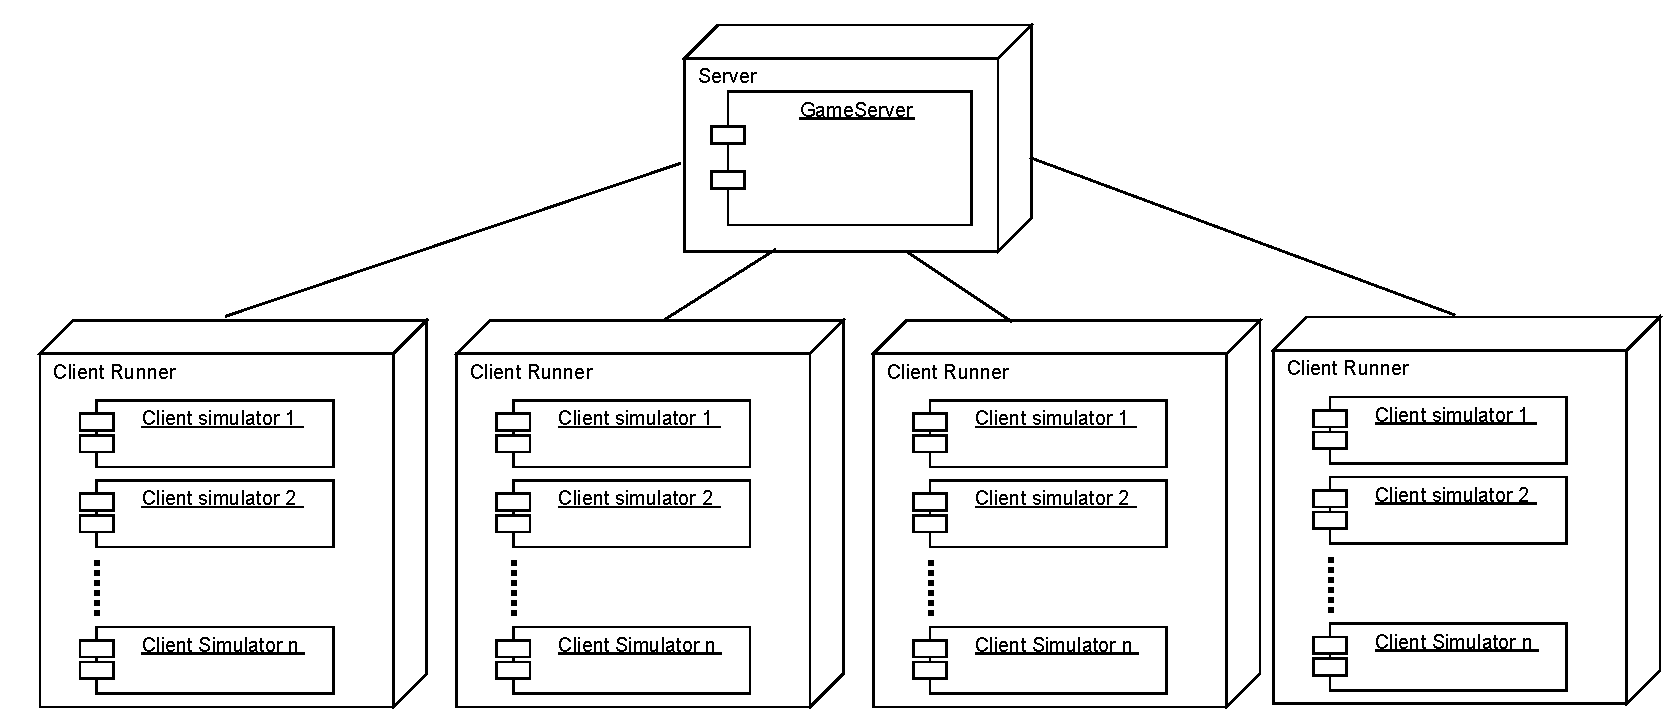
\includegraphics[width=1.0\linewidth]{FIG/DeploymentDiagram.pdf} 
%%   \caption{The
%%     experiments run on one server, with simulated players across multiple machines.}
%\end{figure}
  
To have a realistic behavior of the game clients, the game was run
with 5 human players playing the game with a game update frequency of
10~Hz. The network input to the server from this session was recorded
with a timestamp for each message. The recorded game interactions were
then played back multiple times in parallel to simulate a large number
of clients. To ensure that client performance is not a bottleneck, the
simulated clients were distributed among multiple physical
machines. Furthermore, as an average client generates 2.6~kbps network
traffic, the 1~Gbps local network interface that was used for the
experiments did not limit the performance. The game server was run on a
server machine containing 4 Dual-Core AMD Opteron 8218 (2600~MHz) with
16~GB RAM. To ensure comparable numbers, the server was taken down
between each test run.

\subsection{Response latency}
%
%
%\PH{I think we talked about several ways of discussing latency with different
%types of plots!? I do still think you should include several. One CDF (for a
%given number of clients) that looks at the average response time (not deadline
%misses), and then discuss different latency requirements from this (including
%the corresponding number of deadline missed in the given case) (the different
%latency requirements should be cited to be relevant). Then, a boxplot for each
%number of clients would be good - to show how the the latency changes with the
%number of users. When you reach problems - try to identify what causes the
%problems. }
The most important performance metric for client-server games is response latency from the server. From a player perspective, latency is only visible when it exceeds a certain threshold. Individual peaks in response time are obvious to the players, and will have the most impact on the Quality of Experience, hence we focus on peak values as well as averages in the evaluation.

\begin{figure*}[!t!] 
  \centering
  \subfigure[Single-threaded server]{
    \psfig{file=FIG/boxplot_st.eps, width=6.5cm,angle=-90}
    \label{fig:boxplot_st} 
  }
  \subfigure[Multi-threaded server]{
    \psfig{file=FIG/boxplot_mt.eps,width=6.5cm,angle=-90}
    \label{fig:boxplot_mt}
  }
  \caption{Response time for single- and multi-threaded servers
 (dotted line is the 100~ms threshold). }
  \label{fig:boxPlots}
\end{figure*}

The experiments were run with client numbers ranging from 40 to 800 in
increments of 40, where the goal is to keep the latencies close to the
100~ms QoE threshold for FPS games~\cite{claypool++-2006}. Figure
\ref{fig:boxPlots} shows a box-plot of the response time statistics
from these experiments. All experiments used a pool of 48 worker
threads and distributed the network connections across 8 IP ports.

From these plots, we can see that the single-threaded implementation
is struggling to support 280 players at an average latency close to
100~ms. The median response time is 299~ms, and it already has
extreme values all the way to 860~ms, exceeding the threshold for a good
QoE. The multi-threaded server, on the other hand, is handling the
players well up to 640 players where we are getting samples above 1
second, and the median is at 149~ms.

These statistics are somewhat influenced by the fact that the number of
samples is proportional to the update frequency. This means that long
update cycles to a certain degree get artificially lower weight.

\begin{figure*}[ht]
  \centering 
  \subfigure[400 concurrent clients]{
    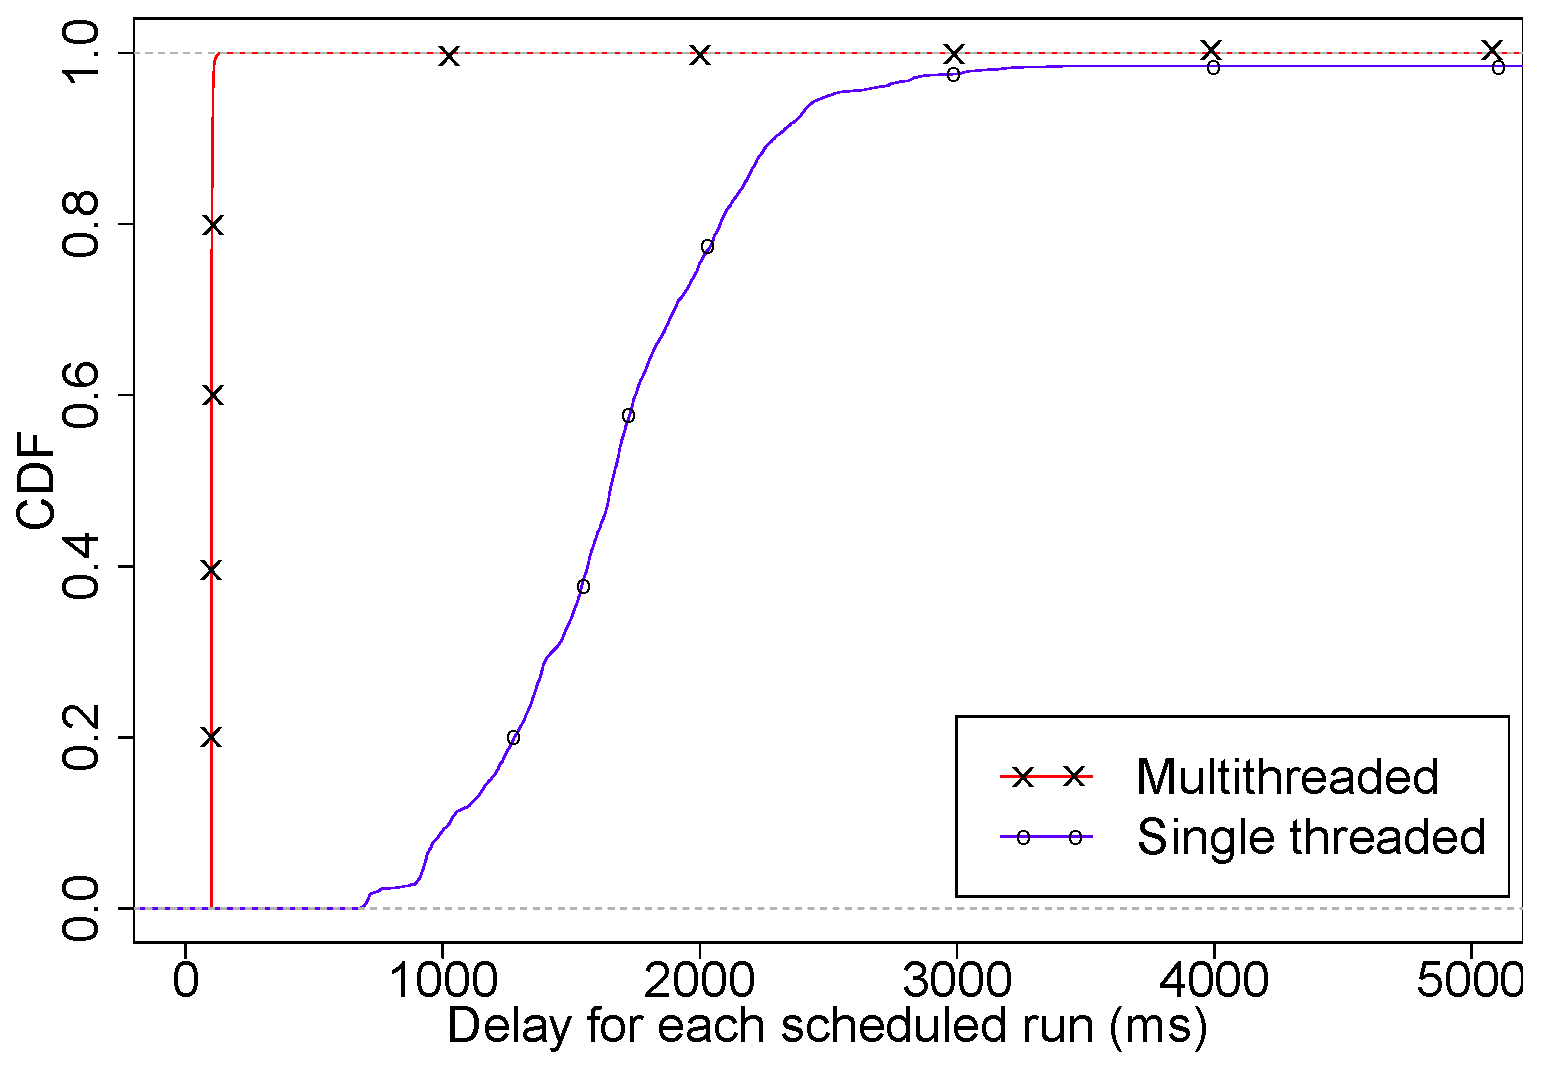
\psfig{file=FIG/cdf-400.eps, width=8.0cm}
    \label{fig:cdf-400}
  }
  \subfigure[800 concurrent clients]{
    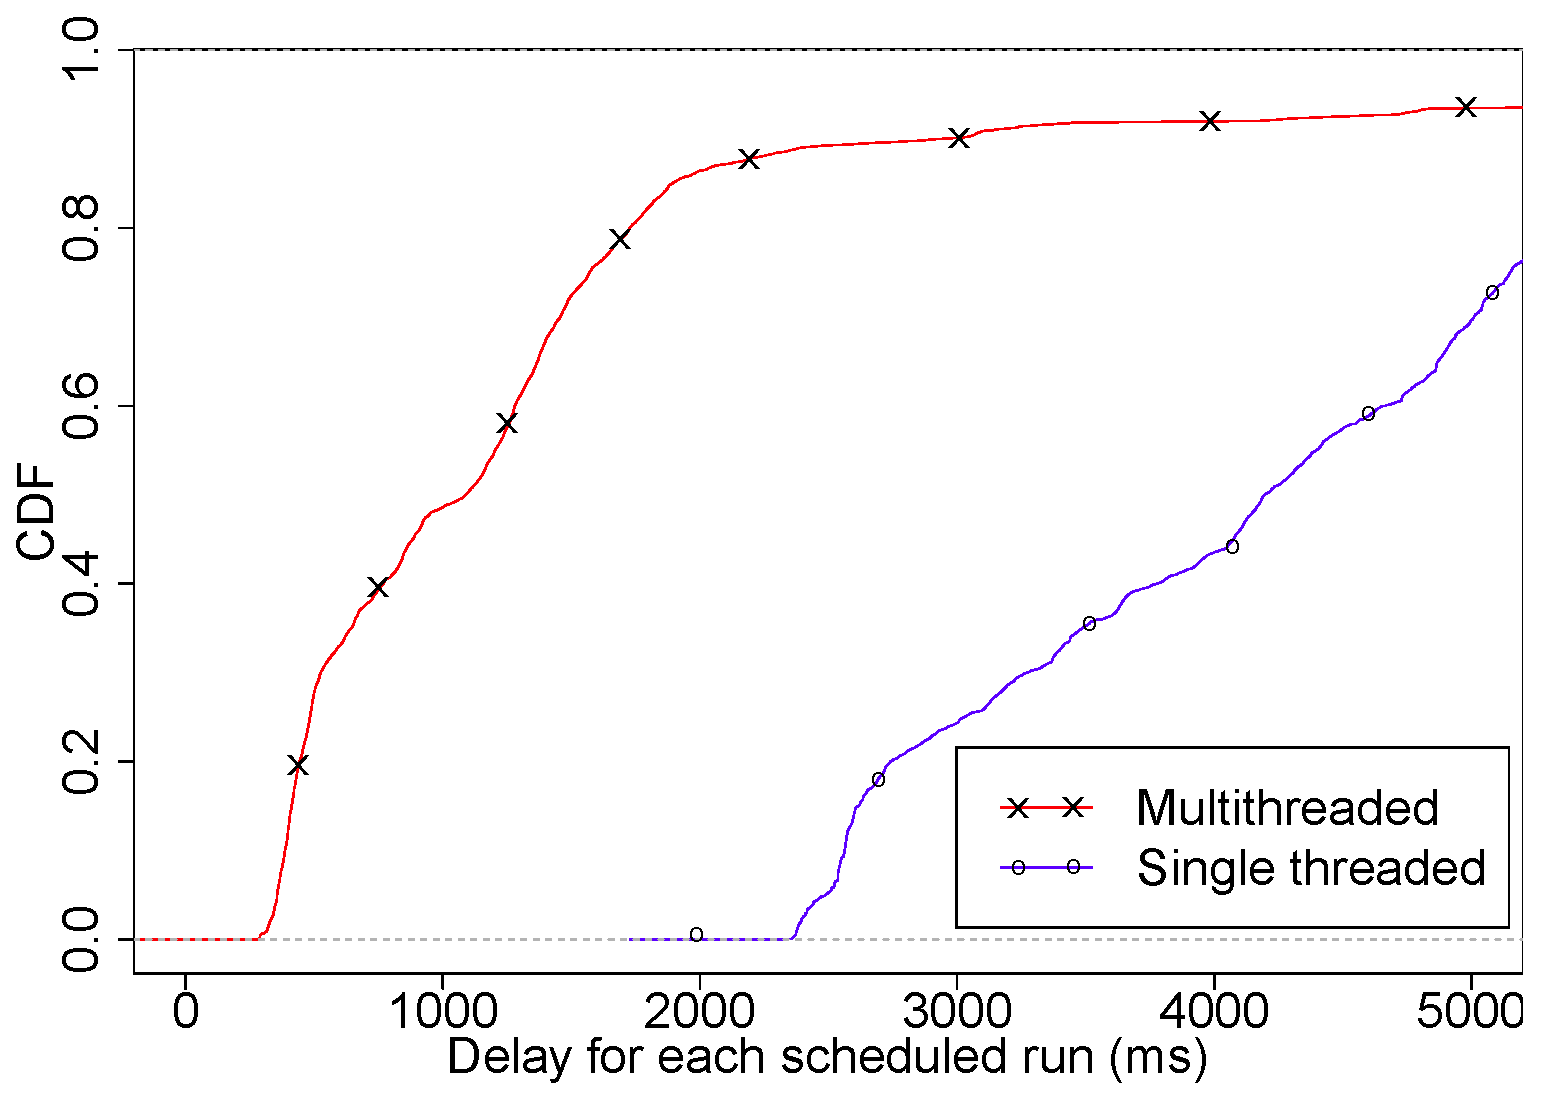
\psfig{file=FIG/cdf-800.eps, width=8.0cm}
    \label{fig:cdf-800}
  }  
%  \vspace{-3mm}
  \caption{CDF of response time for single-  and multi-threaded
    servers with 400 and 800 concurrent clients.}
  \label{fig:CDFPlots}
\end{figure*}

Figure \ref{fig:CDFPlots} shows details of two interesting cases. In
figure \ref{fig:cdf-400}, the single-threaded server is missing all
its deadlines with 400 concurrent players, while the multi-threaded
version is processing almost everything on time. At 800 players
(figure~\ref{fig:cdf-800}), the outliers are going much further for
both cases. Here, even the multi-threaded implementation is struggling
to keep up, though it is still handling the load significantly better
than the single-threaded version, which is generally completely
unplayable.
%\vspace{4mm}
\subsection{Resource consumption}

\begin{figure}
  \centering %\vspace{-3mm}
  \psfig{file=FIG/cpu-load-620-mt.eps,angle=-90, width=\columnwidth} %\vspace{-3mm}
  \caption{CPU load and response time for 620 concurrent clients on
    the multi-threaded server.}
  %\vspace{-3mm} 
  \label{fig:cpu-load-620}
\end{figure}

We have investigated the resource consumption when players connect to
the multhreaded server as shown in figure \ref{fig:cpu-load-620}. We
present the results for 620 players, as this is the highest number of
simultaneous players that server handles before significant
degradation in performance, as shown in figure
\ref{fig:boxplot_mt}. The mean response time is 133~ms, above the
ideal delay of 100~ms. Still, the server is able to keep the update
rate smooth, without significant spikes. The CPU utilization grows
while the clients are logging on, then stabilizes at an almost full
CPU utilization for the rest of the run. The two spikes in response
time happen while new players log in to the server at a very fast rate
(30 clients pr. second). Receiving a new player requires a lock in the
server, hence this operation is, to a certain degree, serial.


\subsection{Effects of thread-pool size}

\begin{figure}
  \centering 
%  \vspace{-3mm}
  \psfig{file=FIG/lineplot-threads.eps,angle=-90, width=\columnwidth}   \caption{Response time for 700 concurrent clients on using varying number of threads. Shaded area from 5 to 95 percentiles.}
%  \vspace{-3mm} 
  \label{fig:line-threads-700}
\end{figure}

To investigate the effects of the number of threads in the threadpool,
we performed an experiment where we kept the number of clients
constant while varying the number of threads in the pool. 700 clients
were chosen, as this number slightly overloads the server. The number of threads in the pool was increased in increments of 2 from 2 to 256. In
figure~\ref{fig:line-threads-700}, we see clearly that the system
utilizes more than 4 cores efficiently, as the 4 thread version shows
significantly higher response times. At one thread per core or more,
the numbers are relatively stable, with a tendency towards more
consistent low response times with more available threads, to about 40
threads. This could mean that threads are occasionally waiting for I/O
operations. Since thread pools are not pre-emptive, such situations
would lead to one core going idle if there are no other available
threads. Too many threads, on the other hand, could lead to excessive
context switch overhead. The results show that the average is slowly increasing after about 50 threads, though the 95-percentile is still decreasing with increased number of threads, up to about 100. From then on the best case is worsening again most likely due to context switching overhead.

A game developer needs to consider this trade-off when tuning the parameters for a specific game.
%\PH{Why the number 700? Use the same number of clients as in figure
%  5!? Can the plot have errorbars instead for the 5/95 percentiles
%  instead of a separate line (it is not intuitive how to read the
%  plot)?  The plot (ot at least the text) should also list the numbers
%for the single-threaded system!!!}

%\PH{Other things to evaluate? Workload per client? Background load? ...}

%% FW: QoE versus resources for reducing/increasing tick length 
%% What is the effect of network latency + server latency
